\documentclass[a4paper]{article}

%%%%%%%% CREATE DOCUMENT STRUCTURE %%%%%%%%
%% Language and font encodings
\usepackage[english]{babel}
\usepackage[utf8x]{inputenc}
\usepackage[T1]{fontenc}
%\usepackage{subfig}

%% Sets page size and margins
\usepackage[a4paper,top=3cm,bottom=2cm,left=2cm,right=2cm,marginparwidth=1.75cm]{geometry}

%% Useful packages
\usepackage{tikz}
\usetikzlibrary{shapes.geometric, arrows}
\usepackage{algorithm} 
\usepackage{algorithmicx} 
\usepackage{algpseudocode}
\usepackage{amsmath}
\usepackage{graphicx}
\usepackage[colorinlistoftodos]{todonotes}
\usepackage[colorlinks=true, allcolors=blue]{hyperref}
\usepackage{caption}
\usepackage{subcaption}
\usepackage{sectsty}
\usepackage{apacite}
\usepackage{float}
\usepackage{titling} 
\usepackage{blindtext}
\usepackage[square,sort,comma,numbers]{natbib}
\usepackage[colorinlistoftodos]{todonotes}
\usepackage{xcolor}
\makeatletter  % Add this!!!!
 \renewcommand{\ALG@name}{Code block} %doesnt work
\makeatother   % Add this also
\renewcommand{\listalgorithmname}{Liste der Pseudocodes}

%%%%%%%% DOCUMENT %%%%%%%%
\begin{document}

%%%% Title Page
\begin{titlepage}

\newcommand{\HRule}{\rule{\linewidth}{0.5mm}} 							% horizontal line and its thickness
\center 
 
% University
\textsc{\LARGE Delft University of Technology}\\[1cm]

% Document info
\textsc{\Large Digital Terrain Modelling}\\[0.2cm]
\textsc{\large GEO1015}\\[1cm] 										% Course Code
\HRule \\[0.8cm]
{ \huge \bfseries Assignment 2: Viewshed Computation}\\[0.7cm]								% Assignment
\HRule \\[1cm]
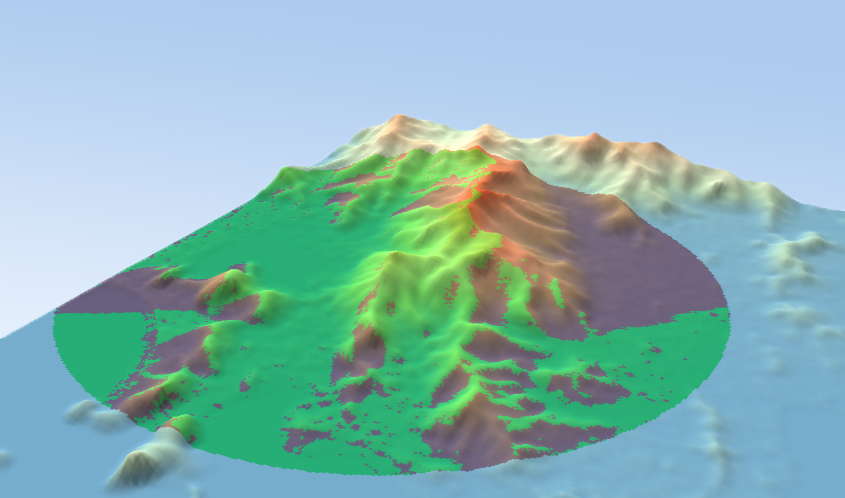
\includegraphics[width=0.8\textwidth]{images/cristo_3d copy.png}\\[1cm]
\large

Michiel de Jong (4376978)\\[1.5cm]													% Author info
{\large \today}\\[2cm]

\includegraphics[width=0.4\textwidth]{images/TU_delft_logo.jpg}\\[1cm] 	% University logo
\vfill 
\end{titlepage}

%%\begin{abstract}
%%Your abstract.
%%\end{abstract}

%%%% SECTIONS
%% Section 1
\section*{General Strategy for Viewshed Computation}
This section will describe step by step the what was done to compute the viewshed analysis. After each step, the relevant parts of the step are illustrated through either pseudocode or a diagram. 

\begin{enumerate}
    \item {\bfseries{Initialize output array and multiple viewpoint handling.}}\newline
    To start everything off, we need to initialize the output array that will be written to file. To make everything easier and faster, I have chosen take an game/explore map approach. This entails that from the outset, everything will be considered invisible, except the viewpoint, until you have seen it. 
    
    To enable the code to handle multiple viewpoints, only the initialisation of the height (input) grid, the visibility (output) grid, and the writing of the file are done outside a loop that iterates over the viewpoints supplied by the .json file.\newline
    
\begin{algorithm}
	\caption{Viewpoint looping} 
	\begin{algorithmic}[1]
	\State $input = $ DEM
	\State $output = $ raster with $shape(input)$ and $values = 3$ \Comment{3 value for outside horizon}
	\State $parameters = $ .json file
		\For {$viewpoint=1,2,\ldots$}
		    \State Compute viewshed analysis around viewpoint
		\EndFor
		\State Write to file using supplied code
	\end{algorithmic} 
\end{algorithm}
    \item{\bfseries{Construct circle based on max viewing distance}}\newline
    To shorten computation times, I have chosen to initiate a circle with the maximum viewing distance as its radius and the viewpoint as its center, and use the cells describing the circumference of that circle as endpoints in Line-of-Sight queries. This is faster, because I only have to consider pixels inside the circles, because all other points are already set to the invisibility value of 3.
    
    The radius is extrapolated through the index of the raster, thus choosing the pixel where the max distance ends, and then using the max distance in "index space" for the construction of the circle. Because the circle is a type of geometry that is not supported by GeoJSON, I had to mathematically construct the circle with the following algorithm. 
\begin{algorithm}
	\caption{Circle construction} 
	\begin{algorithmic}[1]
	\State $r = index[viewpoint_x + maxdistance] - index[viewpoint] $
	\State $center = index[viewpoint]$ 
		\For {$0 < \Theta ≤ 360$}\Comment{To cover all cells between VP and edge}
		    \State $x_{index[point on circle]} = r \cdot \sin{\Theta} + x_{index[viewpoint]}$
		    \State $y_{index[point on circle]} = r \cdot \cos{\Theta} + y_{index[viewpoint]}$
		    \State Add $tuple(x,y)$ to list of cells that describe circle circumference.
		\EndFor
		\State Remove duplicate tuples from list \Comment{Because of increment value}
	\end{algorithmic} 
\end{algorithm}
    \item{\bfseries{Rasterize line with rasterio}}\newline
    The following step is to construct the lines on which the LoS queries will be performed. This is done using a Rasterio module that burns shapes into a raster. The lines are instantiated for each cell in the list of cells that describe the circumference of the max viewing distance circle. Most of this code was already provided, but I will describe it shortly: a GeoJSON LineString is created between the viewpoint(xy) and circle cell (xy). This line is input into the rasterize function, which returns a Boolean array of $shape = input$ with True for the cells which represent the line. This array needs to be converted into a list of cells that will be used to compute the LoS. This is done by determining the lines' position in which quadrant of the circle, and thus sorting it either according to the lines' $x$ or $y$ coordinates.\newpage 
\begin{algorithm}
	\caption{Line rasterization and sorting} 
	\begin{algorithmic}[1]
	\State $input = viewpoint, circlepoint$
		\For {cell, touched by $line[vp, cp]$}
		    \State True
		\EndFor
		\For {$cell == True$}
		    \State add cell to list of cells
		\EndFor
		\If{$line = quadrant_{upperright}$}
		\State sort: x ascending \& y ascending
		\ElsIf{$line = quadrant_{upperleft}$}
		\State sort: x descending \& y ascending
		\ElsIf{$line = quadrant_{lowerright}$}
		\State sort: x ascending \& y descending
		\ElsIf{$line = quadrant_{lowerleft}$}
		\State sort: x descending \& y descending 
		\EndIf
	\end{algorithmic} 
\end{algorithm}   
    \item{\bfseries{Line-of-Sight query}}\newline
    Now we come at the core of the analysis. We arrive at this point with a list of pixels that describes a line between the viewpoint and a point on the circumference created by the circle about the viewpoint with the maximum viewing distance as its radius. The line of sight query is performed using the tangent method. An initial tangent is created between the viewpoint and the first point next to the viewpoint on the line. This tangent is defined by the following equation: $t_{cur}= slope * \Delta x +h_{viewpoint}$,\\
    where $slope =\frac{\Delta h}{\sqrt{\Delta x^2 +\Delta y^2}} $
    and $\Delta x=\sqrt{\Delta x^2 +\Delta y^2}$.\\
    Then for every pixel on the line, the value of $t_{cur}$ is evaluated, and if the value of $t_{cur}$ is equal or lower than the elevation of this pixel, then the pixel is visible, and the tangent is updated with the parameters of this pixel, and the next pixel is evaluated. If the value of $t_{cur}$ is not lower or equal to the elevation of the pixel, the pixel is invisible, and the tangent is not updated.
\begin{algorithm}[H]
	\caption{Line of sight query} 
	\begin{algorithmic}[1]
	\State $t_{cur}= slope * d(viewpoint, pixel_1) +h_{viewpoint}$
	\State $slope =\frac{h_{pixel_1} - x_{viewpoint}}{d(viewpoint,pixel_1}$ 
		\For {pixel in line of sight}
		    \If {$t_{cur} <= h_{pixel}$}
		    \State assign value $[1]$ to pixel
		    \State $slope =\frac{h_{pixel} - x_{viewpoint}}{d(viewpoint, pixel)}$
		    \State $t_{cur}= slope * d(viewpoint, pixel) x +h_{viewpoint}$
		    \Else{}
		    \State assign value $[0]$ to pixel
		    \EndIf
		\EndFor
	\end{algorithmic} 
\end{algorithm}      
In the figure below, there is a visual representation of this procedure. This is a profile of the Tasmania dataset, sliced from (515703.86454456096, 5263772.525086236) to (517705.77522456093, 5263772.525086236). 
\begin{figure}[H]    
\centering
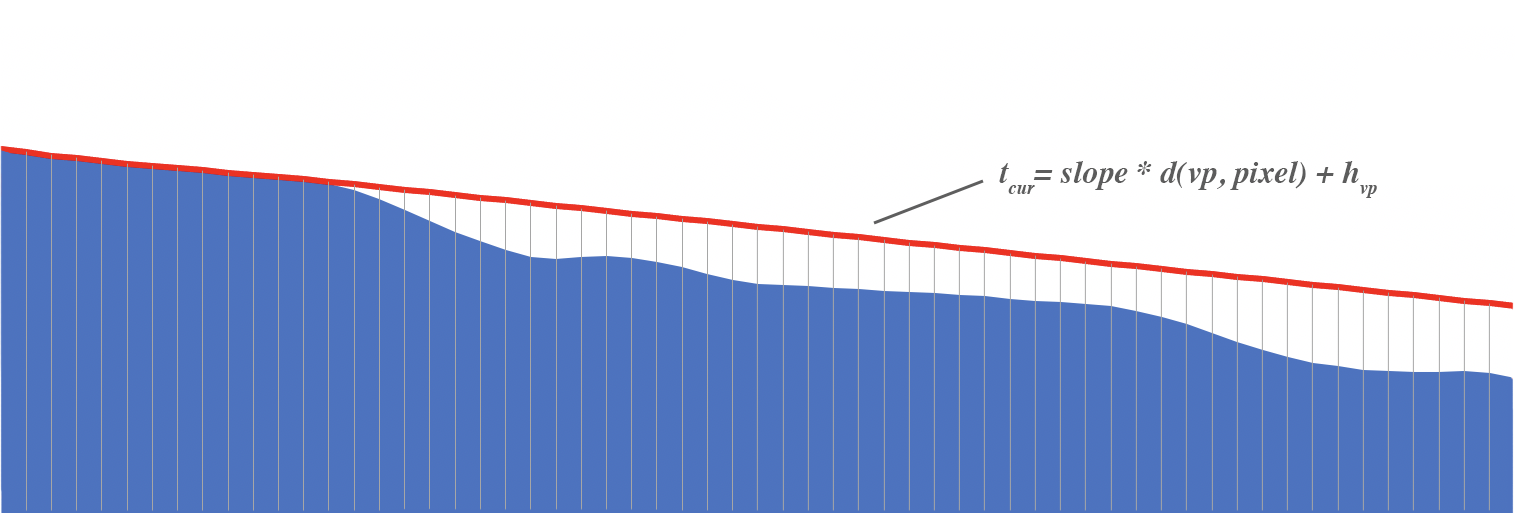
\includegraphics[width = 0.6\textwidth]{images/profile.png}
\caption{Profile with tangent}
\label{fig:tangent}
\end{figure}
\end{enumerate}

\section*{Assumptions made and their consequences}
This section will describe several assumptions, shortcuts and other decisions made in the process that have consequences for the output of the analysis.
\begin{enumerate}
    \item\emph{{Calculation of radius}}\\
    The radius of the circle is calculated in \textit{index space}, thus there is an uncertainty introduced to the viewshed horizon. However, since this is linked to the general resolution of the raster, the effect of this shortcut is generally not high. 
   \begin{algorithm}[H]
	\begin{algorithmic}[1]
	\State \textbf{horizon(x,y)} $= index(x_{viewpoint}+maxdistance,y_{viewpoint}$
	\State \textbf{radius} $= horizon(x,y) - viewpoint(x,y)$
	\end{algorithmic} 
\end{algorithm} 
    \item\emph{{Circle construction \& initial conditions}}\\
    To make sure I only had to deal with the cells that define the \textit{boundary} of the horizon, I decided to construct my circle as described above. This saves me from looping over the entire array, but has to be supported by giving all pixels a value of 3 (outside horizon) from the outset. However, for a discrete computer, a mathematical definition of the circle is not enough, therefore I had to discretize the range, and settled on an increment value of: \[\dfrac{1}{\text{length of the array row}}\]
    This ensures enough "coverage". However, this results in a high number of duplicates for a low maximum viewing distance. This is a trade off that has to be considered. For the Tasmania dataset, the initial statement produces 181800 points on the horizon, but only 480 are needed. For the Cristo dataset, the initial statement produces 224640 points on the horizon, but only 1336 are needed. This could definitely be improved by linking in to a certain discretization factor needed for a specific resolution, because for large dataset this could eventually cost speed instead of save it.
    \begin{figure}[H]    
\centering
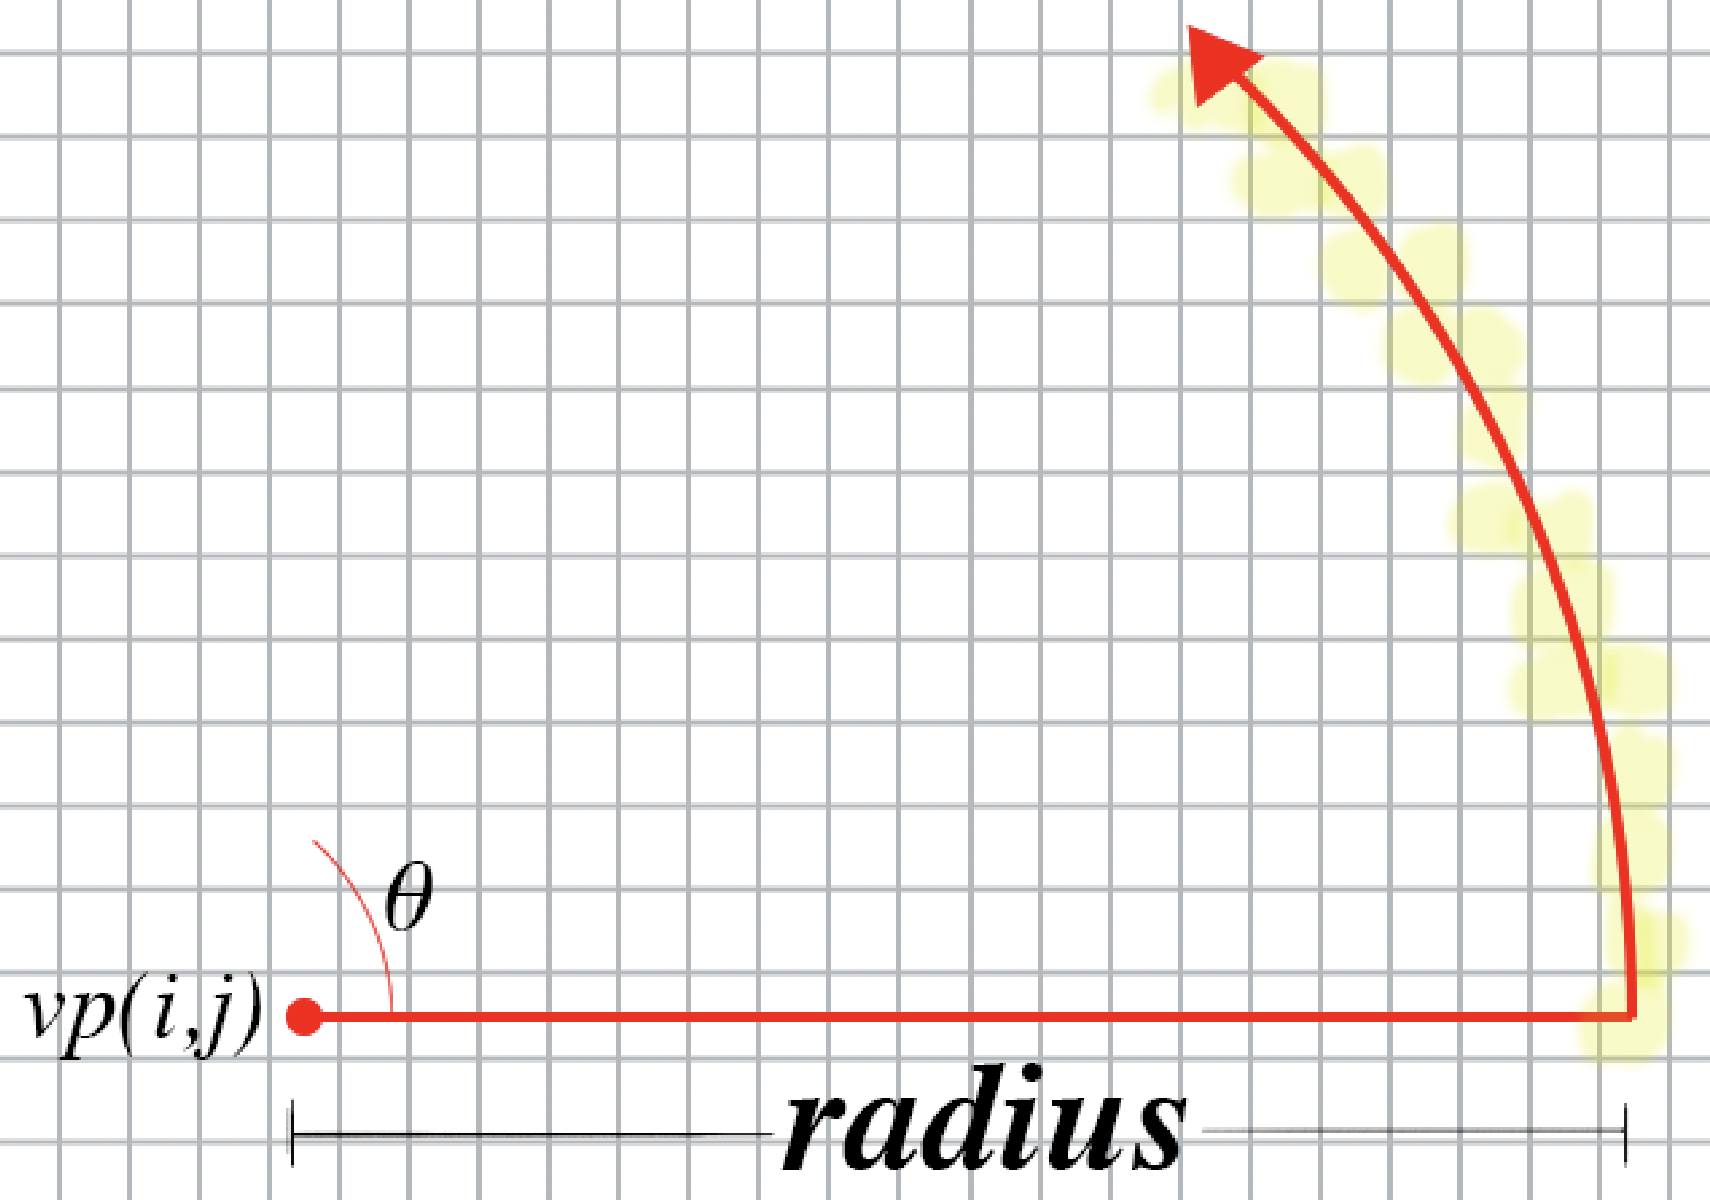
\includegraphics[width = 0.6\textwidth]{images/circle.png}
\caption{Circle construction}
\label{fig:circle}
\end{figure}
\newpage
    \item\emph{{Line rasterization with Rasterio}}\\
    Most of the code to rasterize the viewlines was already present when the code was pulled from GitLab, however, I tweaked some of the presets. Namely, the rasterize function has a parameter \textit{all touched}, which can be true or false. This determines whether \textit{all} pixels that the line touches are being rasterized, or just the pixels whose centers interact with the geometry. This has effect on the viewlines, which can be seen in the figure below. However, due to the fact that when all pixels touched by the line also includes elevations that are not in fact in the line of sight, I have chosen to use the stricter definition, with only pixels whose center is within the polygon or that are selected by Bresenham’s line algorithm used. This also has a benefit for speed, because per viewline, less pixels need to be evaluated.  
\begin{figure}[H]    
\centering
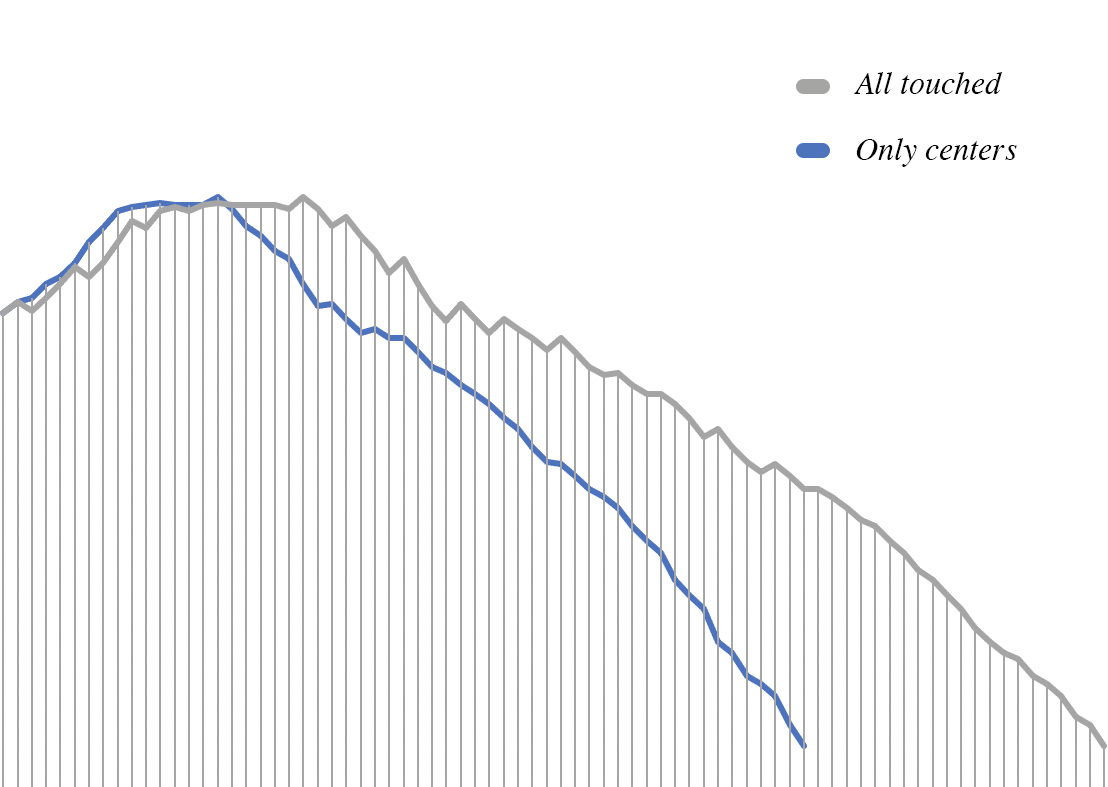
\includegraphics[width = 0.7\textwidth]{images/pixelscomp.png}
\caption{Comparison of profiles with different parameters}
\label{fig:profilecomp}
\end{figure}
    \item\emph{{Multiple visibility's}}\\
    Another thing I had to take into account was that, especially near the center, when most of the viewlines share their pixels. To speed this all up, only pixels that have not already been "seen" by the algorithm are included for the line of sight query. Because if a pixel can be seen in one of the lines of sight, it can be seen in all the lines of sight (lines of sight do not go around the corner).
\begin{algorithm}[H]
	\begin{algorithmic}[1]
	\If{$value_{pixel} \neq 1$ and $value_{pixel} \neq 2$}
	\State include pixel with LoS query
	\EndIf
	\end{algorithmic} 
\end{algorithm}  
    This way, less pixels will be passed for LoS calculation by the algorithm, which will decrease running time. Furthermore, this approach also helps with multiple viewpoints. Otherwise the second viewpoints would just overwrite what the first viewpoint has calculated, which is not what is required, which is: if one DTM cell is visible only from one viewpoint, then it is visible.
\end{enumerate}
\newpage
\section*{Results, benchmarking and validation}
To validate the results, I have done multiple comparisons with the "Profile Tool" plugin in QGIS, which show an accurate result for the viewshed analysis. 
\begin{figure}[H]    
\centering
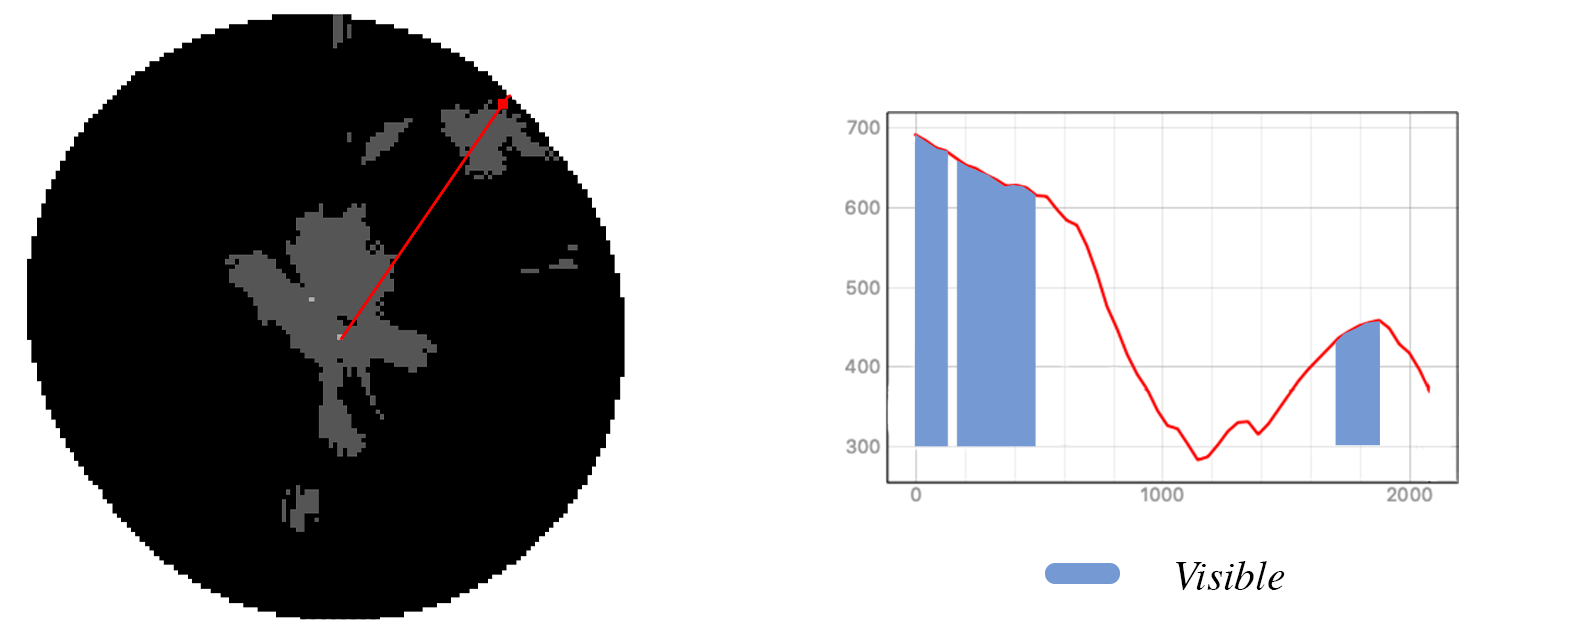
\includegraphics[width = 0.8\textwidth]{images/profile_tool copy.png}
\caption{Comparison of viewshed analysis and profile extracted from DEM.}
\label{fig:profiletool}
\end{figure}
The figure above shows a intuitively correct result. 
Of course, the GeoTIFF's will be supplied with the report. 
Secondly, all these measures to speed up things seem to have worked, for the write times are not high.\\
For the Tasmania dataset:
\begin{verbatim}
Viewshed file written to 'out-tasmania.tif'
--- 2.745 seconds ---     
\end{verbatim}
And for the Cristo dataset:
\begin{verbatim}
Viewshed file written to 'out-cristo.tif'
--- 7.179 seconds ---
\end{verbatim}
Lastly, all is documented on:
\url{https://github.com/dumigil/viewshed_computation}

%%%%%%%% EXTRA TIPS %%%%%%%%
%% hou deze structuur aan voor afbeeldingen
%%\begin{figure}[H]
%%\includegraphics[]{Pendulum.jpg}
%%\caption{Sketch of the pendulum}
%%\label{fig:pendulum}
%%\end{figure}


%%\newpage
%%\bibliographystyle{apacite}
%%\bibliography{sample}

\end{document}